\chapter{Genética do Desenvolvimento e Evolução da Forma}\label{ch:b3:developmental-genetics}

O ovo de uma mosca-das-frutas tem meio milímetro de comprimento e, nas
três horas após a fecundação, antes que uma única membrana celular tenha
se formado entre seus seis mil núcleos, ele decide que extremidade será
a cabeça, qual a cauda, onde ficará cada um de catorze segmentos e quais
deles terão pernas, asas ou antenas. Ele o faz com algumas dezenas de
genes, ligados numa hierarquia de faixas cada vez mais finas, cada faixa
lida a partir das concentrações dos produtos das faixas anteriores. Em
1980 dois jovens cientistas em Heidelberg rastrearam milhares de moscas
mutantes em busca de larvas com partes faltando ou duplicadas, e
encontraram toda a hierarquia: genes cuja perda apaga um bloco de
segmentos, genes cuja perda apaga um segmento sim e outro não, genes
cuja perda vira todo segmento de trás para a frente. O trabalho do mesmo
ano sobre um gene que transforma o terceiro segmento de uma mosca numa
cópia do segundo --- dando-lhe quatro asas, como tinham seus ancestrais
--- abriu um conjunto de genes mestres que, veio a se descobrir,
ficavam na mesma ordem ao longo dos cromossomos de um camundongo e de um
humano, e faziam o mesmo trabalho. Este capítulo trata de como um embrião
computa sua própria geometria, de como algumas centenas de genes
regulatórios constroem todo corpo animal, e de como mudar quando e onde
eles agem produziu a diversidade da forma animal.

\section{As coordenadas da mosca}

\begin{definition}[A hierarquia da segmentação]\label{def:b3:developmental-genetics:hierarchy}
\index{gene de efeito materno}\index{gene gap}\index{gene pair-rule}\index{gene de polaridade segmentar}\index{blastoderma sincicial}
O embrião de \emph{Drosophila} se desenvolve, em suas primeiras treze
divisões nucleares, como um \emph{blastoderma sincicial}, uma única
célula cujos núcleos compartilham um citoplasma, de modo que as
proteínas se difundem livremente a partir de onde são feitas. Quatro
gradientes estabelecidos pelas células da mãe fixam os eixos: o mRNA de
\emph{bicoid} fica ancorado no polo anterior e sua proteína se difunde
para trás formando um gradiente exponencial da cabeça à cauda; o mRNA de
\emph{nanos}, no polo posterior, faz o gradiente espelhado; os mRNAs de
\emph{hunchback} e \emph{caudal} são uniformes, mas a proteína Bicoid
reprime a tradução de \emph{caudal} e a Nanos reprime a de
\emph{hunchback}, de modo que suas proteínas também formam gradientes.
Esses produtos de \emph{efeito materno}, cujo fenótipo mutante depende
do genótipo da mãe e não do embrião, ligam os \emph{genes gap}
(\emph{hunchback}, \emph{Krüppel}, \emph{knirps}, \emph{giant}) em
faixas largas, cada uma respondendo a uma faixa de concentração de
Bicoid e reprimindo suas vizinhas; as proteínas gap, em combinação,
ligam os \emph{genes pair-rule} (\emph{even-skipped}, \emph{fushi
tarazu}, \emph{hairy}) em sete faixas cada, alternadas; e as proteínas
pair-rule ligam os \emph{genes de polaridade segmentar}
(\emph{engrailed}, \emph{wingless}, \emph{hedgehog}) em catorze faixas,
uma por segmento, que fixam a frente e o fundo de cada segmento e são
mantidas, depois que as células se formam, pela sinalização entre elas.
Três horas, quatro níveis, de um único gradiente a catorze segmentos ---
e os nomes dos mutantes registram o rastreamento: \emph{hunchback} não
tem tórax, \emph{Krüppel} (``aleijado'') não tem o meio, \emph{fushi
tarazu} (``segmentos insuficientes'') não tem um segmento sim e outro
não, \emph{hedgehog} tem um gramado de cerdas.
\end{definition}

\begin{omfigure}
\begin{tikzpicture}[every node/.style={font=\scriptsize}, >=stealth]
  \foreach \y/\lab/\n in {0/{materno: gradiente de Bicoid}/1, -1.3/{genes gap: 4 faixas largas}/2, -2.6/{genes pair-rule: 7 faixas}/3, -3.9/{polaridade segmentar: 14 faixas}/4} {
    \draw[thick, gray!60] (0,\y) ellipse (3.6 and 0.5);
    \node[left, align=right] at (-3.8,\y) {\lab};
  }
  % bicoid gradient shading
  \begin{scope}
    \clip (0,0) ellipse (3.6 and 0.5);
    \shade[left color=omDef!80, right color=omDef!2] (-3.6,-0.5) rectangle (3.6,0.5);
  \end{scope}
  \node[right, font=\tiny] at (3.7,0) {alto na frente};
  % gap bands
  \begin{scope}
    \clip (0,-1.3) ellipse (3.6 and 0.5);
    \fill[omDef!50] (-3.4,-1.8) rectangle (-1.6,-0.8); \fill[omThm!40] (-1.4,-1.8) rectangle (0.2,-0.8); \fill[omMeth!40] (0.4,-1.8) rectangle (1.7,-0.8); \fill[omProp!45] (1.9,-1.8) rectangle (3.4,-0.8);
  \end{scope}
  \node[font=\tiny] at (-2.5,-1.3) {\emph{hb}}; \node[font=\tiny] at (-0.6,-1.3) {\emph{Kr}}; \node[font=\tiny] at (1.05,-1.3) {\emph{kni}}; \node[font=\tiny] at (2.65,-1.3) {\emph{gt}};
  % pair-rule stripes
  \begin{scope}
    \clip (0,-2.6) ellipse (3.6 and 0.5);
    \foreach \i in {0,...,6} { \fill[omThm!50] ({-3.1+\i*0.9},-3.1) rectangle ({-2.75+\i*0.9},-2.1); }
  \end{scope}
  \node[right, font=\tiny] at (3.7,-2.6) {\emph{eve}, um segmento sim, outro não};
  % segment polarity stripes
  \begin{scope}
    \clip (0,-3.9) ellipse (3.6 and 0.5);
    \foreach \i in {0,...,13} { \fill[omProp!60] ({-3.25+\i*0.47},-4.4) rectangle ({-3.1+\i*0.47},-3.4); }
  \end{scope}
  \node[right, font=\tiny] at (3.7,-3.9) {\emph{en}: um por segmento};
  \foreach \y in {-0.55,-1.85,-3.15} { \draw[->, thick] (0,\y) -- (0,\y-0.2); }
  \node[below, align=center, font=\tiny] at (0,-4.5) {cada nível lê as concentrações do nível acima;\\três horas de um único gradiente a catorze segmentos};
\end{tikzpicture}

{\small A hierarquia da segmentação. Um gradiente materno é lido em
quatro faixas de \omterm{def:b3:developmental-genetics:hierarchy}{genes gap}; as proteínas gap, em combinação, em sete
faixas pair-rule; e estas, em catorze faixas de polaridade segmentar.
Cada faixa é um limite traçado onde uma concentração cruza um limiar.}
\end{omfigure}

\begin{theorem}[Um gradiente de morfógeno a partir de síntese, difusão e degradação]\label{thm:b3:developmental-genetics:gradient}
\index{morfógeno}\index{informação posicional}\index{modelo da bandeira francesa}\index{comprimento de decaimento}
Uma proteína feita numa extremidade de um tecido à taxa $J$ (por unidade
de área), que se difunde com coeficiente $D$ e é degradada com constante
de taxa $k$, alcança um regime estacionário em que sua concentração ao
longo do eixo $x$ obedece a
\[
D\,\frac{\mathrm{d}^{2}c}{\mathrm{d}x^{2}} - k\,c = 0,
\qquad c(x) = c_{0}\,\mathrm{e}^{-x/\lambda}, \qquad \lambda = \sqrt{D/k},
\quad c_{0} = \frac{J}{\sqrt{Dk}} .
\]
O \emph{\omterm{thm:b3:developmental-genetics:gradient}{comprimento de decaimento}} $\lambda$ fixa o alcance do
gradiente; uma célula lê sua posição comparando $c$ com limiares --- a
\emph{bandeira francesa} de Wolpert (1969): acima de $T_{1}$, azul;
entre $T_{1}$ e $T_{2}$, branco; abaixo, vermelho --- e o limite para o
limiar $T$ fica em $x_{T} = \lambda\ln(c_{0}/T)$. Duas consequências:
dobrar a fonte desloca todo limite para trás pelo mesmo $\lambda\ln 2$,
e um erro fracionário $\delta c/c$ na leitura da concentração é um erro
posicional $\delta x = \lambda\,\delta c/c$, de modo que um gradiente só
consegue colocar um limite com precisão de uma célula se as células o
lerem com precisão de alguns por cento. A Bicoid tem $\lambda \approx \qty{100}{\micro m}$ num ovo de \qty{500}{\micro m}: o gradiente abrange
um fator $\mathrm{e}^{5}
\approx 150$, e o limite de \emph{hunchback}
fica no meio do ovo, onde a Bicoid caiu a cerca de um doze avos de seu
pico.
\end{theorem}
\begin{proof}
Conservação numa fatia entre $x$ e $x + \mathrm{d}x$: a entrada difusiva
líquida $D\,\partial^{2}c/\partial x^{2}$ equilibra a degradação $kc$ em
regime estacionário, dando a equação; a solução limitada quando $x \to \infty$ é a exponencial decrescente com $\lambda^{2} = D/k$. A fonte: o
fluxo difusivo em $x = 0$, $-D\,
c'(0) = Dc_{0}/\lambda$, é igual a $J$,
de modo que $c_{0} = J\lambda/D =
J/\sqrt{Dk}$. Limiar:
$c_{0}\mathrm{e}^{-x_{T}/\lambda} = T$ dá $x_{T}$; dobrar $c_{0}$
acrescenta $\lambda\ln 2$ a todo $x_{T}$, seja qual for $T$. Erro:
derivando $x_{T} = \lambda\ln(c_{0}/c)$, $\delta x = -\lambda\,\delta c/c$. O regime estacionário é alcançado na escala de tempo $1/k$, que
para a Bicoid (\qty{50}{min}) é comparável às duas horas disponíveis, de
modo que o gradiente é lido enquanto ainda se acomoda.
\end{proof}

\begin{omfigure}
\begin{tikzpicture}
\begin{axis}[
  width=0.7\linewidth, height=5.6cm,
  axis x line=bottom, axis y line=left,
  xmin=0, xmax=500, ymin=0, ymax=1.05,
  xlabel={distância do polo anterior (\unit{\micro m})}, ylabel={Bicoid, relativa},
  xlabel style={font=\small, at={(axis description cs:0.5,-0.12)}, anchor=north}, ylabel style={font=\small},
  tick label style={font=\small}, xtick={0,100,250,400,500}, ytick={0.08,0.3,0.6,1},
  yticklabels={0.08,0.3,0.6,1},
  clip=false,
]
\fill[omDef!15] (axis cs:0,0) rectangle (axis cs:120,1.05);
\fill[gray!8] (axis cs:120,0) rectangle (axis cs:250,1.05);
\fill[omThm!12] (axis cs:250,0) rectangle (axis cs:500,1.05);
\addplot[very thick, omDef, domain=0:500, samples=100] {exp(-x/100)};
\addplot[thick, omDef!50, dashed, domain=66:500, samples=100] {2*exp(-x/100)};
\draw[dashed, gray] (axis cs:0,0.3) -- (axis cs:120,0.3) -- (axis cs:120,0);
\draw[dashed, gray] (axis cs:0,0.08) -- (axis cs:250,0.08) -- (axis cs:250,0);
\node[font=\scriptsize, anchor=south] at (axis cs:60,1.0) {cabeça};
\node[font=\scriptsize, anchor=south] at (axis cs:185,1.0) {tórax};
\node[font=\scriptsize, anchor=south] at (axis cs:375,1.0) {abdome};
\node[font=\scriptsize, omDef, anchor=west] at (axis cs:255,0.35) {$c = c_{0}\,\mathrm{e}^{-x/\lambda}$, $\lambda = \qty{100}{\micro m}$};
\node[font=\scriptsize, omDef!70!black, anchor=west, align=left] at (axis cs:255,0.62) {tracejado: fonte dobrada ---\\todo limite se desloca $\lambda\ln 2 = \qty{69}{\micro m}$};
\node[font=\scriptsize, gray, anchor=north east] at (axis cs:118,0.29) {$T_{1}$};
\node[font=\scriptsize, gray, anchor=south west] at (axis cs:300,0.09) {$T_{2}$: \emph{hunchback} desligado};
\end{axis}
\end{tikzpicture}

{\small A bandeira francesa traçada por uma exponencial. Limiares sobre
um único gradiente repartem o ovo em regiões; uma fonte mais forte move
todos os limites para trás pela mesma distância, que é o que mostram os
embriões de mães com cópias extras de \emph{bicoid}.}
\end{omfigure}

\begin{proof}[Evidência]
Nüsslein-Volhard e Wieschaus (1980) alimentaram moscas com um mutagênico,
cruzaram os descendentes até a homozigose e olharam ao microscópio as
cutículas de umas \num{27000} larvas mortas em busca de padrões faltando
ou repetidos: cerca de cento e vinte genes, classificados por seus
fenótipos nas classes gap, pair-rule e de polaridade segmentar --- uma
hierarquia visível antes que se conhecesse molécula alguma. Driever e
Nüsslein-Volhard (1988) coraram embriões para a proteína Bicoid e viram
o gradiente exponencial a partir do polo anterior; embriões de mães com
uma, duas, quatro ou seis cópias do gene tinham gradientes de altura
proporcional, e a prega cefálica e o limite de \emph{hunchback} se
moviam para trás com a dose, como o modelo de limiar prevê, e
aproximadamente pelo $\lambda\ln 2$ por duplicação que ele exige.
Injetar mRNA de \emph{bicoid} no meio de um ovo produzia ali uma cabeça.
\end{proof}

\begin{omfigure}
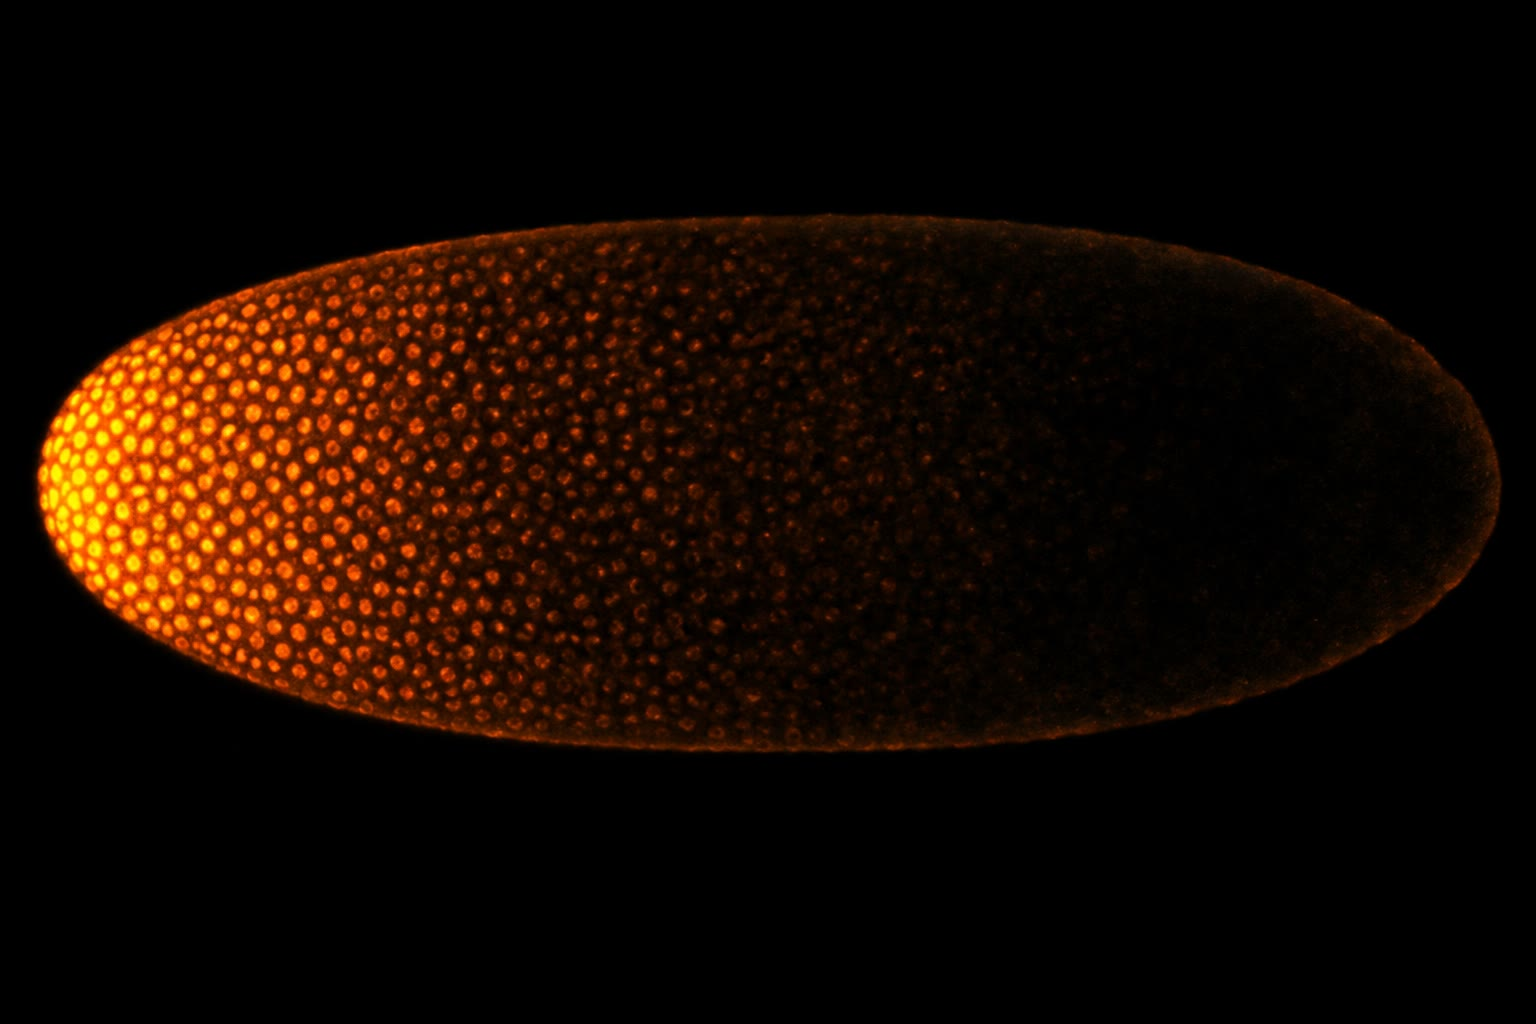
\includegraphics[width=0.46\linewidth]{images/book5/ai/b5-23-bicoid-gradient.jpg}\hspace{0.04\linewidth}
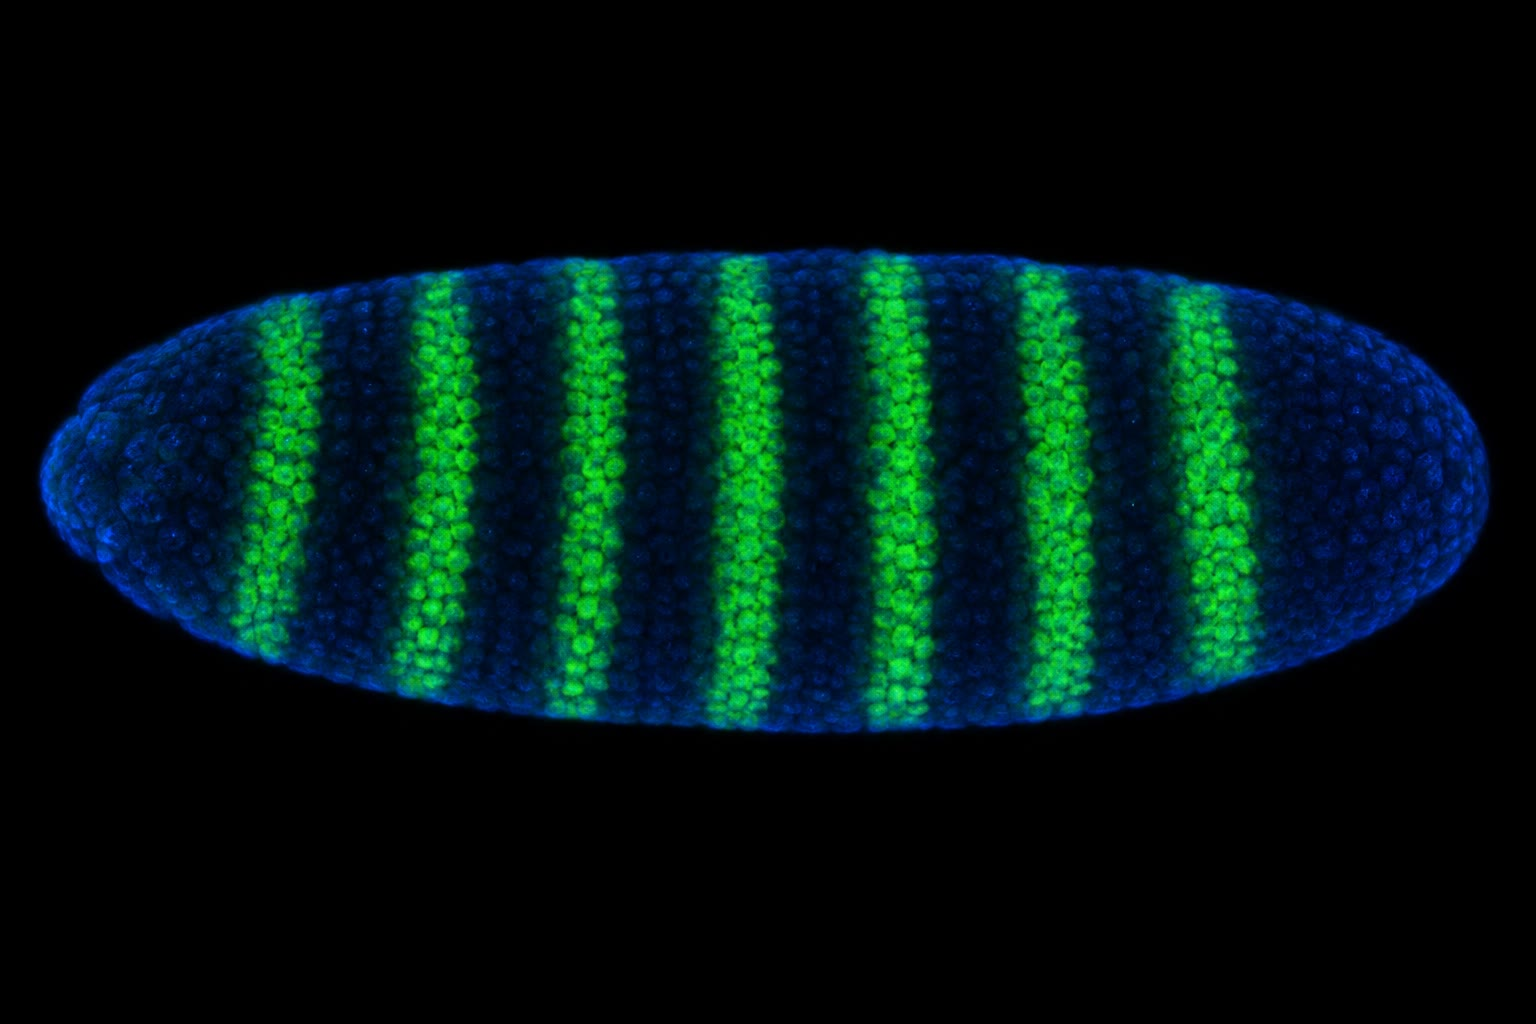
\includegraphics[width=0.46\linewidth]{images/book5/ai/b5-23-embryo-stripes.jpg}

{\small À esquerda: um embrião sincicial corado para a proteína Bicoid,
mais brilhante no polo anterior e desvanecendo exponencialmente rumo ao
posterior. À direita: um embrião uma hora depois, corado para uma
proteína pair-rule, sete faixas traçadas a partir das faixas dos \omterm{def:b3:developmental-genetics:hierarchy}{genes
gap}.}
\end{omfigure}

\section{Identidade: os genes Hox}

\begin{definition}[Genes homeóticos e colinearidade]\label{def:b3:developmental-genetics:hox}
\index{mutação homeótica}\index{genes Hox}\index{colinearidade}\index{homeobox}\index{código Hox}
Uma mutação \emph{homeótica} transforma uma parte do corpo em outra: a
palavra é de Bateson (1894) para as anormalidades que ``substituem um
membro de uma série por outro''. Na mosca, os mutantes dominantes
\emph{Antennapedia} fazem crescer pernas onde deveria haver antenas; os
mutantes \emph{bithorax} (Lewis, 1978) transformam o terceiro segmento
torácico numa cópia do segundo, de modo que os balancins (halteres)
viram um segundo par de asas. Os oito genes responsáveis, os \emph{genes
Hox}, ficam em dois agrupamentos de um mesmo cromossomo, e Lewis notou
que sua ordem ao longo do DNA corresponde à ordem, ao longo do corpo,
dos segmentos que eles controlam --- a \emph{colinearidade}, ainda não
totalmente explicada. Cada um codifica um fator de transcrição com o
mesmo domínio \emph{homeobox} de ligação ao DNA, de 60 aminoácidos
(McGinnis, Gehring, 1984), que foi então encontrado em todo animal:
camundongos e humanos carregam quatro agrupamentos de treze genes cada,
colineares do mesmo modo, expressos em domínios aninhados ao longo do
eixo do corpo, com os genes mais tardios do agrupamento mais
posteriores. A identidade de uma célula ao longo do eixo é dada pela
combinação de genes Hox que ela expressa, o \emph{código Hox}; os genes
posteriores dominam os anteriores (prevalência posterior), de modo que
perder um gene posterior deixa o segmento adotar a identidade do que
está à frente. Os genes Hox não constroem um segmento; eles dizem a um
segmento já construído qual segmento ele é, ligando as baterias de genes
a jusante apropriadas a uma perna, uma asa, uma costela ou uma vértebra
lombar.
\end{definition}

\begin{omfigure}
\begin{tikzpicture}[every node/.style={font=\scriptsize}, >=stealth]
  % fly cluster
  \node[left] at (-0.3,2.2) {mosca (\emph{Drosophila}), 8 genes};
  \foreach \i/\g/\c in {0/lab/omDef, 1/pb/omDef, 2/Dfd/omThm, 3/Scr/omThm, 4/Antp/omMeth, 5/Ubx/omMeth, 6/abd-A/omProp, 7/Abd-B/omProp} {
    \draw[thick, fill=\c!40] ({\i*1.1},1.9) rectangle ({\i*1.1+0.9},2.5); \node[font=\tiny] at ({\i*1.1+0.45},2.2) {\emph{\g}};
  }
  \node[left] at (-0.3,0.9) {agrupamento HoxB do camundongo, 9 de 13};
  \foreach \i/\g/\c in {0/b1/omDef, 1/b2/omDef, 2/b3/omDef, 3/b4/omThm, 4/b5/omThm, 5/b6/omMeth, 6/b7/omMeth, 7/b8/omProp, 8/b9/omProp} {
    \draw[thick, fill=\c!40] ({\i*1.1},0.6) rectangle ({\i*1.1+0.9},1.2); \node[font=\tiny] at ({\i*1.1+0.45},0.9) {\emph{\g}};
  }
  \draw[->, thick] (0,1.55) -- (9.8,1.55); \node[above, font=\tiny] at (4.9,2.55) {3$'$ $\to$ 5$'$ ao longo do DNA};
  \draw[->, thick] (0,0.2) -- (9.8,0.2); \node[below, font=\tiny] at (4.9,0.05) {anterior $\to$ posterior ao longo do corpo};
  % body schematic
  \node[left] at (-0.3,-0.9) {expressos em};
  \draw[thick, gray!70, rounded corners=6pt] (0,-1.3) rectangle (9.8,-0.5);
  \foreach \x/\t in {0.6/cabeça, 2.6/pescoço, 4.4/tórax, 6.6/lombar, 8.6/{sacral, cauda}} { \node[font=\tiny] at (\x,-0.9) {\t}; }
  \draw[gray!70] (1.6,-1.3) -- (1.6,-0.5); \draw[gray!70] (3.5,-1.3) -- (3.5,-0.5); \draw[gray!70] (5.6,-1.3) -- (5.6,-0.5); \draw[gray!70] (7.6,-1.3) -- (7.6,-0.5);
  \node[below, align=center, font=\tiny] at (4.9,-1.4) {colinearidade: a ordem dos genes no cromossomo é a de seus domínios no corpo;\\os mesmos agrupamentos, a mesma ordem, da mosca ao camundongo ---\\herdados de um ancestral de 600 milhões de anos atrás};
\end{tikzpicture}

{\small Agrupamentos Hox numa mosca e num camundongo. Os genes ficam ao
longo do DNA na ordem das regiões do corpo que especificam, nos dois
animais, e os genes homólogos podem ser reconhecidos pela sequência: um
gene \emph{Hoxb6} de camundongo é reconhecivelmente o
\emph{Antennapedia} da mosca.}
\end{omfigure}

\begin{proof}[Evidência]
Lewis (1978) mapeou o complexo \emph{bithorax} como uma série de
mutações, cada uma transformando um segmento no que está à frente,
dispostas no cromossomo na ordem do corpo, e propôs que os genes eram
ativados sequencialmente ao longo do eixo. McGinnis e colaboradores
(1984) encontraram o \omterm{def:b3:developmental-genetics:hox}{homeobox} por hibridização cruzada entre
\emph{Antennapedia} e \emph{Ultrabithorax} e depois em rãs e camundongos.
A equivalência funcional foi mostrada diretamente: um gene \emph{Hoxb6}
de camundongo expresso numa mosca produz o fenótipo
\emph{Antennapedia}, pernas no lugar de antenas (anos 1990); um
camundongo sem \emph{Hoxc8} tem uma costela extra em sua primeira
vértebra lombar, tendo o segmento assumido a identidade do que está à
frente; e alterar os limites de expressão Hox em galinha e camundongo
desloca a posição em que se formam os membros anteriores, sendo o
comprimento do pescoço de um cisne acompanhado por um deslocamento
posterior do mesmo limite.
\end{proof}

\begin{omfigure}
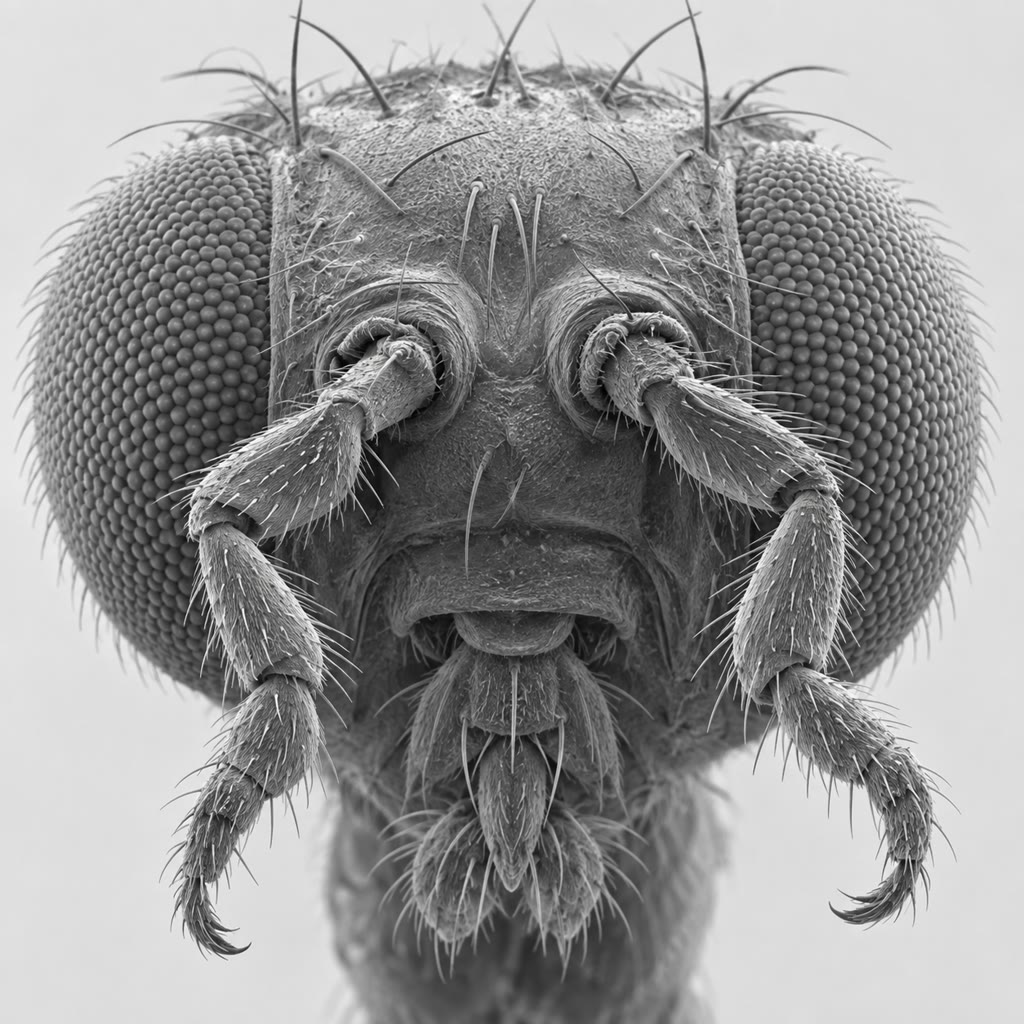
\includegraphics[width=0.34\linewidth]{images/book5/ai/b5-23-antennapedia-fly.jpg}\hspace{0.04\linewidth}
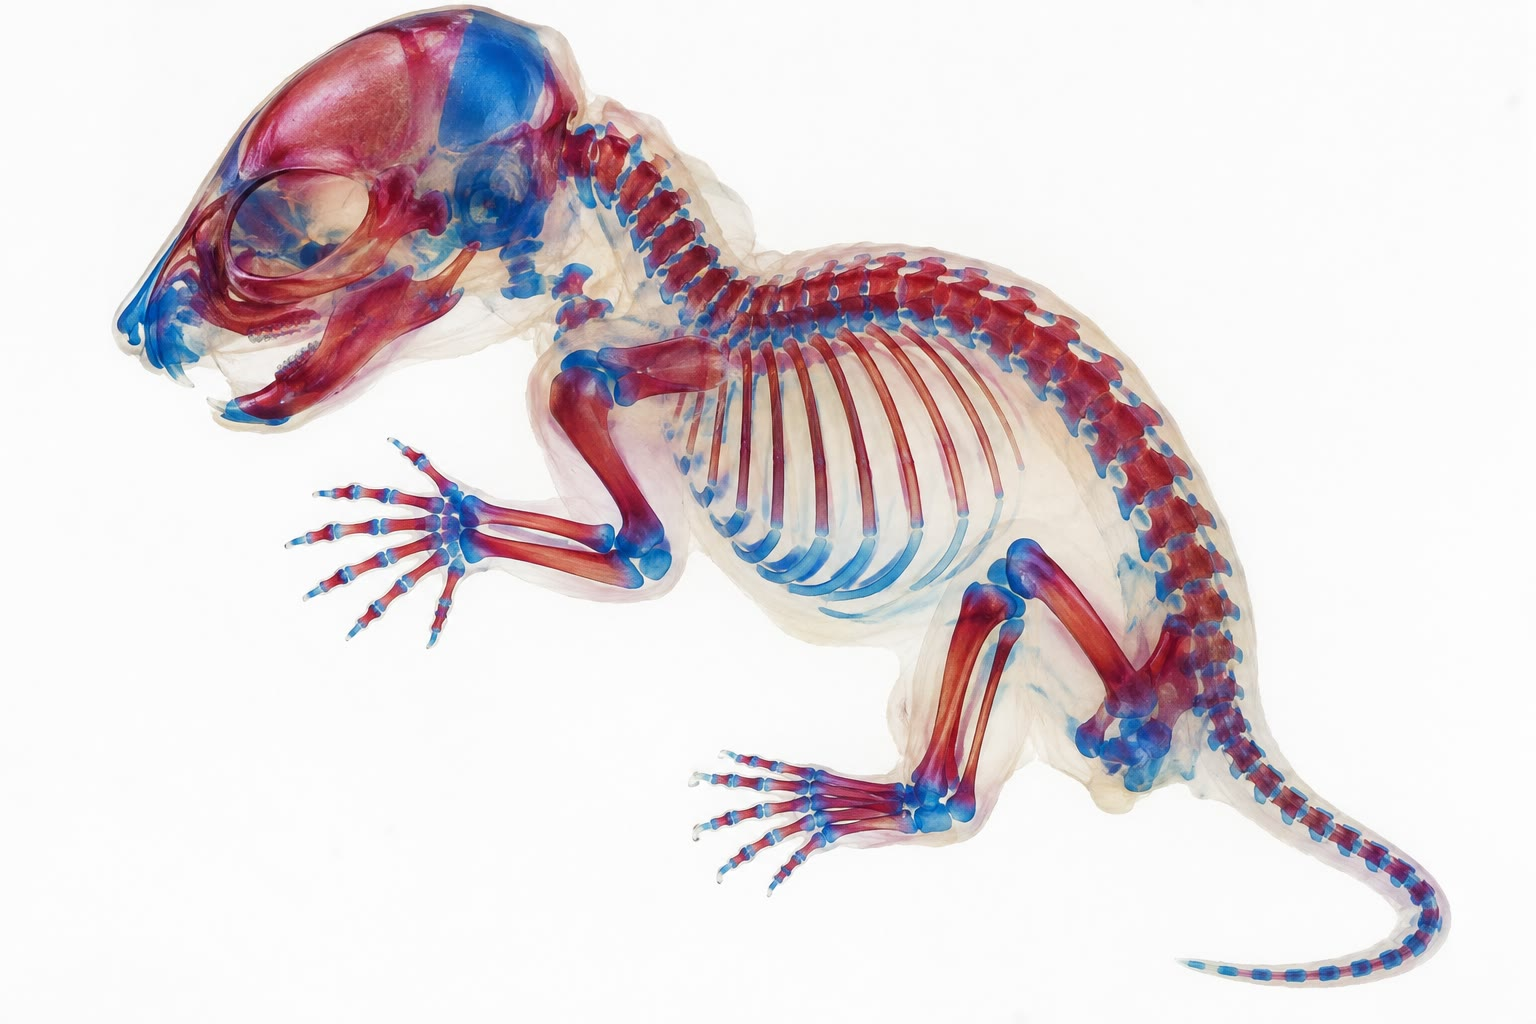
\includegraphics[width=0.5\linewidth]{images/book5/ai/b5-23-limb-skeleton-stain.jpg}

{\small À esquerda: a cabeça de uma mosca mutante \emph{Antennapedia}, um
par de pernas onde deveria haver antenas --- o segmento construído
corretamente e informado da identidade errada. À direita: o esqueleto de
um embrião de camundongo, cartilagem em azul e osso em vermelho, as
vértebras ao longo das quais o \omterm{def:b3:developmental-genetics:hox}{código Hox} é lido.}
\end{omfigure}

\section{Construir um vertebrado}

\begin{definition}[Organizadores e centros de sinalização]\label{def:b3:developmental-genetics:organiser}
\index{organizador}\index{indução}\index{sonic hedgehog}\index{broto do membro}\index{zona de atividade polarizadora}\index{crista ectodérmica apical}
Os embriões de vertebrados são celulares desde o início, de modo que
seus gradientes são feitos por proteínas secretadas, e não pela difusão
de um sincício, e as mesmas poucas famílias fazem tudo: Wnt, Hedgehog,
BMP e outros parentes do TGF-$\beta$, FGF, Notch e ácido retinoico.
Spemann e Mangold (1924) enxertaram um pedaço do lábio dorsal de uma
gástrula de tritão no ventre de outra e obtiveram um segundo embrião, da
cabeça à cauda, feito sobretudo de células do hospedeiro: o enxerto era
um \emph{organizador}, que induzia seus vizinhos a formar um sistema
nervoso e um eixo, e suas moléculas se revelaram, setenta anos depois,
antagonistas secretados (Chordin, Noggin) que bloqueiam a BMP, cuja
ausência permite que o ectoderma se torne neural --- o padrão. O
\emph{tubo neural} é então padronizado dorsoventralmente pelo
\emph{sonic hedgehog} da notocorda e da placa do assoalho (alto:
neurônios motores; baixo: \omterm{def:b3:nervous-systems:cells}{interneurônios}) contra a BMP do teto; e o
\emph{broto do membro}, por dois centros, a \emph{zona de atividade
polarizadora} em sua margem posterior, que secreta Shh (cujo enxerto na
margem anterior dá uma duplicação em espelho dos dedos, seis dedos se
encontrando polegar com polegar), e a \emph{crista ectodérmica apical}
em sua ponta, que secreta FGFs que mantêm em divisão as células
subjacentes e especificam a sequência proximal-distal de úmero,
antebraço e mão. Enxerto, ablação e esferas embebidas em proteína
continuam sendo as ferramentas; a lógica --- uma fonte local, um
gradiente, limiares, um código de fatores de transcrição --- é a da
mosca.
\end{definition}

\begin{omfigure}
\begin{tikzpicture}[every node/.style={font=\scriptsize}, >=stealth]
  % limb bud
  \fill[omDef!12] (0,0) -- (0,3) .. controls (2.6,3.4) and (3.4,2.2) .. (3.4,1.5) .. controls (3.4,0.8) and (2.6,-0.4) .. (0,0) -- cycle;
  \draw[thick, omDef] (0,0) -- (0,3) .. controls (2.6,3.4) and (3.4,2.2) .. (3.4,1.5) .. controls (3.4,0.8) and (2.6,-0.4) .. (0,0);
  \draw[very thick, omMeth!70!black] (2.9,2.5) .. controls (3.45,1.9) and (3.45,1.1) .. (2.9,0.5);
  \node[right, align=left, omMeth!70!black, font=\tiny] at (3.5,1.5) {crista ectodérmica apical:\\FGF8; mantém a\\zona de progresso em divisão;\\proximal $\to$ distal};
  \begin{scope}
    \clip (0,0) -- (0,3) .. controls (2.6,3.4) and (3.4,2.2) .. (3.4,1.5) .. controls (3.4,0.8) and (2.6,-0.4) .. (0,0) -- cycle;
    \foreach \i/\op in {1/50, 2/38, 3/26, 4/14} { \draw[omThm!\op, thick] (0.6,0.5) circle ({0.45*\i}); }
  \end{scope}
  \fill[omThm!50] (0.6,0.5) ellipse (0.5 and 0.35); \node[anchor=north, align=center, omThm, font=\tiny] at (0.9,-0.2) {ZPA: sonic hedgehog,\\posterior $\to$ anterior};
  \node[left, font=\tiny] at (-0.05,2.6) {anterior}; \node[left, font=\tiny] at (-0.05,0.4) {posterior};
  \node[left, font=\tiny] at (-0.05,1.5) {parede do corpo};
  \draw[->, thick] (0.3,1.5) -- (3.0,1.5); \node[above, font=\tiny] at (1.75,1.55) {úmero, antebraço, dedos};
  % right: digit code
  \node[right, align=left] at (7.2,2.6) {identidade do dedo pela exposição a Shh:\\polegar (dedo 1): nenhuma;\\dedos 2--3: gradiente;\\dedos 4--5: de células que expressam Shh};
  \node[right, align=left] at (7.2,1.0) {enxerte uma segunda ZPA na frente:\\duplicação em espelho, 4-3-2-2-3-4;\\uma esfera com proteína Shh faz o mesmo};
  \node[right, align=left, gray] at (7.2,-0.2) {a mesma molécula padroniza o tubo neural\\(neurônios motores onde ela é alta) e o intestino};
\end{tikzpicture}

{\small Os dois centros de sinalização do \omterm{def:b3:developmental-genetics:organiser}{broto do membro}. O \omterm{def:b3:developmental-genetics:organiser}{sonic
hedgehog} da margem posterior diz às células que dedo se tornarem; o FGF
da ponta lhes diz quão longe estão ao longo do membro. Enxertos que
movem um centro movem o padrão com ele.}
\end{omfigure}

\begin{proposition}[Padrão espontâneo: o mecanismo de Turing]\label{prop:b3:developmental-genetics:turing}
\index{padrão de Turing}\index{reação--difusão}\index{ativador--inibidor}
Nem todo padrão é lido de um gradiente preexistente. Turing (1952)
mostrou que duas substâncias que se difundem e reagem --- um
\emph{ativador} que estimula sua própria produção e a de um
\emph{inibidor}, e um inibidor que suprime o ativador e se difunde muito
mais depressa --- podem transformar espontaneamente um campo uniforme
num arranjo regular de picos: um pequeno excesso local de ativador cresce
por autorreforço enquanto o inibidor que ele produz se espalha e impede
que novos picos se formem por perto, de modo que os picos surgem num
espaçamento fixado pelo alcance do inibidor, $\lambda \sim \sqrt{D_{\text{inib}}/k_{\text{inib}}}$, e não por coordenada externa
alguma. O mecanismo, aqui admitido em sua matemática, é a melhor
explicação para as manchas e listras dos pelames, para o espaçamento dos
folículos pilosos e dos brotos de pena, para as cristas do palato, para
os dedos da mão (cujo número sobe quando o comprimento de onda do padrão
é encurtado pela redução da atividade Hox) e para as listras do
peixe-zebra, em que as células que interagem --- células pigmentares que
repelem vizinhas de um tipo e atraem as de outro a distância --- foram
identificadas e suas listras, levadas a se refazer após ablação a laser
exatamente como a teoria prevê.
\end{proposition}
\admitted

\section{Evolução da forma}

\begin{definition}[Evo-devo]\label{def:b3:developmental-genetics:evodevo}
\index{homologia profunda}\index{kit de ferramentas genético}\index{evolução cis-regulatória}\index{heterocronia}
Os genes que constroem os animais são um \emph{kit de ferramentas}
antigo e compartilhado: algumas centenas de fatores de transcrição e
vias de sinalização já presentes no ancestral comum de todos os animais,
e a diversidade animal vem sobretudo de mudanças em \emph{quando, onde e
quanto} eles são expressos, e não no que codificam. \emph{Homologia
profunda}: o gene \emph{Pax6} dirige a formação do olho em moscas, lulas
e camundongos, cujos olhos não são homólogos como órgãos --- um
\emph{Pax6} de camundongo expresso na perna de uma mosca faz ali um olho
de mosca ectópico (Halder, Gehring, 1995). \emph{Evolução
cis-regulatória}: a perda dos espinhos pélvicos nos esgana-gatas de água
doce é a deleção de um único intensificador do gene \emph{Pitx1}, com a
proteína intacta e ainda servindo em outros lugares; a perda das manchas
das asas em algumas moscas-das-frutas, uma mudança num intensificador de
\emph{yellow}; a perda das pernas nas cobras, um intensificador
quebrado de \emph{\omterm{def:b3:developmental-genetics:organiser}{sonic hedgehog}} no membro. \emph{Deslocamentos Hox}: o
limite de expressão de \emph{Hoxc6} marca a primeira vértebra torácica
igualmente em camundongo, galinha, ganso e cobra, nas vértebras 7, 14,
23 e 3; a perda das pernas abdominais nos insetos foi a proteína Hox Ubx
adquirindo um domínio repressor que desliga o gene da perna
\emph{Distal-less}, onde nos crustáceos ela não o faz. A
\emph{heterocronia}, uma mudança no tempo de um programa de
desenvolvimento, fez do axolote uma larva permanente e do rosto humano o
de um macaco juvenil. A velha pergunta de como surgem formas novas vira
uma pergunta sobre DNA regulatório: a maior parte do genoma que importa
para a forma não é gene, é interruptor.
\end{definition}

\begin{example}[Quatro asas]\label{ex:b3:developmental-genetics:four-wings}
Os ancestrais das moscas tinham quatro asas, como libélulas e abelhas
ainda têm; as moscas têm duas, com o par posterior reduzido aos
balancins. Nas moscas, \emph{Ultrabithorax} é expresso no terceiro
segmento torácico e ali reprime o programa da asa --- uns cem genes-alvo,
sendo um halter uma asa com esses genes desligados. A mosca mutante
tripla de Lewis, sem função de \emph{Ubx} no terceiro segmento, faz
crescer um segundo par de asas: não uma estrutura nova, mas a liberação
de uma antiga. Nas borboletas o \emph{Ubx} é expresso também na asa
posterior e, ali, não suprime a asa, mas muda seu padrão: a mesma
proteína, um conjunto diferente de alvos. Quatrocentos milhões de anos de
evolução dos dípteros dependeram da decisão de um gene num segmento, e
uma única mutação a desfaz numa geração --- e é por isso que a história
da forma é legível nos genes que a constroem.
\end{example}

\begin{remark}[Geometria a partir da química]\label{rem:b3:developmental-genetics:remark}
Um embrião não tem planta nem agrimensor. Ele tem alguns gradientes
feitos por difusão e degradação, células que os leem contra limiares e
ligam fatores de transcrição, e um código desses fatores que diz a cada
região o que se tornar; tem \omterm{def:b3:developmental-genetics:organiser}{organizadores} locais que induzem seus
vizinhos, e reações que se padronizam sozinhas. A matemática é a da
cinética de primeira ordem e da difusão --- uma exponencial, uma raiz
quadrada, um limiar --- e ela explica não só como a cabeça de uma mosca é
posicionada, mas por que dobrar um gene desloca um limite por uma
distância fixa, por que aparecem seis dedos quando um sinal é duplicado,
e por que uma cobra tem trezentas costelas. A evolução edita os
interruptores, e não a máquina: o kit de ferramentas de uma esponja e o
de um humano são quase o mesmo, e o que difere é a fiação.
\end{remark}

\section{Exercícios}

\begin{exercise}[$\star$]\label{exo:b3:developmental-genetics:1}
Nomeie os quatro níveis da hierarquia de segmentação da mosca, um gene
de cada e o fenótipo mutante que o colocou em sua classe.
\end{exercise}

\begin{exercise}[$\star$]\label{exo:b3:developmental-genetics:2}
O que é um \omterm{def:b3:developmental-genetics:hierarchy}{gene de efeito materno}? Uma fêmea homozigota para uma mutação
nula de \emph{bicoid} é cruzada com um macho selvagem: descreva seus
embriões e explique por que o genótipo deles não os salva.
\end{exercise}

\begin{exercise}[$\star$]\label{exo:b3:developmental-genetics:3}
Enuncie a \omterm{def:b3:developmental-genetics:hox}{colinearidade} e a prevalência posterior. Preveja o fenótipo de
um camundongo sem \emph{Hoxc8} e o de uma mosca que expressa
\emph{Antennapedia} na cabeça.
\end{exercise}

\begin{exercise}[$\star$]\label{exo:b3:developmental-genetics:4}
O que o enxerto de Spemann--Mangold mostrou, e que moléculas se
descobriu serem as do \omterm{def:b3:developmental-genetics:organiser}{organizador}? Por que o destino neural é chamado
de ``padrão''?
\end{exercise}

\begin{exercise}[$\star\star$]\label{exo:b3:developmental-genetics:5}
Bicoid: $D = \qty{4}{\micro m^2/s}$, meia-vida de \qty{35}{min}. Calcule
$k$, $\lambda$ e a razão entre as concentrações no polo anterior e no
meio do ovo (\qty{250}{\micro m}).
\end{exercise}

\begin{exercise}[$\star\star$]\label{exo:b3:developmental-genetics:6}
Com $\lambda = \qty{100}{\micro m}$, um limite fica em
\qty{240}{\micro m}. Onde ele fica se a mãe carregar quatro cópias de
\emph{bicoid} em vez de duas? E uma cópia? Expresse os deslocamentos
como fração de um ovo de \qty{500}{\micro m}.
\end{exercise}

\begin{exercise}[$\star\star$]\label{exo:b3:developmental-genetics:7}
Os núcleos do blastoderma estão a \qty{8}{\micro m} um do outro. Para
colocar um limite com precisão de um núcleo, com $\lambda = \qty{100}{\micro m}$, com que precisão um núcleo precisa ler a
concentração de Bicoid? Se o núcleo contar moléculas ao longo de um
tempo $\tau$ e a contagem for de Poisson, quantas ele precisa contar?
\end{exercise}

\begin{exercise}[$\star\star$]\label{exo:b3:developmental-genetics:8}
O gradiente se aproxima do regime estacionário na escala de tempo $1/k$.
Com uma meia-vida de \qty{35}{min}, que fração da concentração
estacionária é alcançada em \qty{60}{min}, \qty{90}{min} e
\qty{120}{min}? O que isso implica para um embrião que precisa ler o
gradiente até \qty{150}{min}?
\end{exercise}

\begin{exercise}[$\star\star$]\label{exo:b3:developmental-genetics:9}
Uma ZPA é enxertada na margem anterior de um broto de membro de galinha.
Preveja o padrão dos dedos, e o padrão se, em vez disso, for implantada
ali uma esfera que libera uma dose baixa de Shh.
\end{exercise}

\begin{exercise}[$\star\star\star$]\label{exo:b3:developmental-genetics:10}
Um morfógeno é feito por todo um tecido de comprimento $L$ à taxa $s$ por
unidade de volume, degradado à taxa $k$ e destruído no limite $x =
L$ (um
sorvedouro absorvente), sem fluxo em $x = 0$. Resolva $Dc'' - kc + s =
0$
para $c(x)$ e esboce-o. Em que a forma desse gradiente difere do caso da
fonte numa extremidade, e o que acontece quando $L \ll \lambda$?
\end{exercise}

\begin{exercise}[$\star\star\star$]\label{exo:b3:developmental-genetics:11}
Dois limiares em $T_{1} = 0.3c_{0}$ e $T_{2} = 0.08c_{0}$ dividem um
gradiente em três regiões. Mostre que as larguras das duas primeiras
regiões não dependem de $c_{0}$, e explique por que um embrião cujo
\emph{comprimento} varia entre indivíduos (de \qty{450}{} a
\qty{550}{\micro m}) precisa de algo mais que uma simples exponencial
para escalonar seu padrão. Proponha um mecanismo.
\end{exercise}

\begin{exercise}[$\star\star\star$]\label{exo:b3:developmental-genetics:12}
Os esgana-gatas perderam os espinhos pélvicos deletando um
intensificador de \emph{Pitx1}; as cobras perderam os membros quebrando
um intensificador de \emph{\omterm{def:b3:developmental-genetics:organiser}{sonic hedgehog}}. Explique por que mudanças
regulatórias, e não mudanças codificantes, são a rota usual para uma
estrutura perdida ou alterada, em termos de pleiotropia e do que a mesma
proteína faz em outros lugares.
\end{exercise}

\section{Problema: A Bandeira Francesa}

\begin{problem}[{Problema de fim de semana --- o sistema de coordenadas
de um ovo calculado a partir da cinética de primeira ordem: o
comprimento, a fonte e o tempo de formação do gradiente de Bicoid, os
limites que ele traça e sua precisão, o que a dosagem gênica e o tamanho
do ovo fazem com eles, e o código Hox lido a jusante, terminando no
comprimento de decaimento, no deslocamento por duplicação e na precisão
posicional}]
\label{pb:b3:developmental-genetics:1}
Dados: comprimento do ovo \qty{500}{\micro m}; Bicoid $D = \qty{4}{\micro m^2/s}$,
meia-vida de \qty{35}{min}; fluxo da fonte tal que $c_{0} = \qty{50}{nM}$
com duas cópias maternas; espaçamento nuclear \qty{8.5}{\micro m} no
ciclo 14; limiares $T_{1} = 0.3\,c_{0}$ (cabeça/tórax) e $T_{2} =
0.08\,c_{0}$ (limite de \emph{hunchback}) para o caso de duas cópias.
Ruído de leitura $\delta c/c = 0.1$ para um único núcleo. Número de
Avogadro \qty{6e23}{}; um núcleo é uma esfera de raio \qty{3}{\micro m}.

\medskip
\noindent\textbf{Parte I --- O gradiente.}
\begin{enumerate}
  \item Calcule $k$ a partir da meia-vida, em \unit{s^{-1}}, e o tempo
        de vida $1/k$ em minutos.
  \item Calcule $\lambda = \sqrt{D/k}$ em micrômetros. Quantos
        \omterm{thm:b3:developmental-genetics:gradient}{comprimentos de decaimento} tem o ovo?
  \item A concentração cai por que fator de um polo ao outro? E por que
        fator ao longo de um espaçamento nuclear no meio do ovo?
  \item Calcule o fluxo da fonte $J = c_{0}\sqrt{Dk}$ em
        \unit{nM\,\micro m\,s^{-1}}, e o número de moléculas que entram
        por segundo num trecho de \qty{1}{\micro m^2} do polo anterior.
  \item Número de moléculas de Bicoid num núcleo do polo ($c_{0}$) e no
        meio do ovo.
  \item Fração do regime estacionário alcançada em \qty{60}{min} e
        \qty{120}{min} ($1 - \mathrm{e}^{-kt}$). O gradiente está
        estacionário quando os limites são traçados, por volta de
        \qty{120}{min}?
\end{enumerate}

\medskip
\noindent\textbf{Parte II --- Limites.}
\begin{enumerate}[resume]
  \item Posições dos dois limites, em \unit{\micro m} e como frações do
        comprimento do ovo.
  \item A mãe tem quatro cópias: novo $c_{0}$ e as duas posições dos
        limites. De quanto cada um se moveu? E com seis cópias?
  \item Uma cópia: posições. Que regiões cresceram e quais encolheram?
  \item Erro posicional a partir de um ruído de leitura de \qty{10}{\%},
        em micrômetros e em espaçamentos nucleares.
  \item Se o erro precisa ser de um núcleo, que precisão de leitura é
        necessária? Se o núcleo tira a média de $n$ leituras
        independentes e o ruído cai como $1/\sqrt{n}$, quantas leituras?
  \item Um núcleo no limite de \emph{hunchback} contém o número
        calculado na questão~5. Qual é o ruído de Poisson $1/\sqrt{N}$ de
        uma única contagem instantânea? Compare com \qty{10}{\%} e
        comente.
\end{enumerate}

\medskip
\noindent\textbf{Parte III --- Escalonamento e robustez.}
\begin{enumerate}[resume]
  \item Os ovos variam de \qty{450}{} a \qty{550}{\micro m}. Se $\lambda$
        e $c_{0}$ forem fixos, onde cai o limite de \emph{hunchback} como
        fração do comprimento do ovo em cada caso? O padrão está
        escalonado?
  \item Suponha, em vez disso, que $D$ escale como $L^{2}$ (o mesmo tempo
        de vida, mas uma fonte cujo espalhamento cresce com o ovo).
        Mostre que $\lambda/L$ é então constante e o padrão escalona.
        Isso é plausível?
  \item O gene \emph{hunchback} responde à Bicoid com um \omterm{def:b3:structural-biology:allostery}{coeficiente de
        Hill} de $5$: sua expressão é $c^{5}/(c^{5} + T^{5})$. Ao longo de
        quantos micrômetros a expressão vai de \qty{10}{\%} a
        \qty{90}{\%} em torno do limite? Compare com um espaçamento
        nuclear.
  \item Explique por que uma resposta íngreme afia um limite mas não
        reduz, por si só, o erro posicional devido ao ruído de
        concentração.
  \item A repressão mútua entre \omterm{def:b3:developmental-genetics:hierarchy}{genes gap} afia e estabiliza seus limites.
        Argumente numa frase por que dois genes que se reprimem
        mutuamente não podem estar ambos ligados no mesmo núcleo em
        regime estacionário.
  \item A temperatura eleva $D$ em \qty{2}{\%} e $k$ em \qty{6}{\%} por
        grau. Variação de $\lambda$ por grau, e o deslocamento do limite
        numa sala \qty{5}{\celsius} mais quente. Por que os embriões
        podem precisar de um mecanismo compensatório?
\end{enumerate}

\medskip
\noindent\textbf{Parte IV --- Identidade.}
\begin{enumerate}[resume]
  \item O \omterm{def:b3:developmental-genetics:hox}{código Hox}: com oito \omterm{def:b3:developmental-genetics:hox}{genes Hox} de mosca, cada um ligado ou
        desligado, quantos códigos são possíveis? Quantos são usados
        (catorze segmentos)? Por que a prevalência posterior reduz o
        número efetivo?
  \item Uma mosca não tem \emph{Ubx} em seu terceiro segmento torácico. O
        que o segmento se torna, e por que o resultado são quatro asas e
        não uma estrutura nova?
  \item O limite de \emph{Hoxc6} de um camundongo fica na vértebra 7, e o
        de um ganso na 23. O que isso prevê sobre seus pescoços, e o que
        mudou na evolução: o gene ou sua expressão?
  \item Um enxerto de ZPA dá dedos 4-3-2-2-3-4. Explique o padrão a
        partir de dois gradientes de Shh que se encontram no meio.
  \item Halder e Gehring expressaram \emph{Pax6} de camundongo na perna
        de uma mosca e obtiveram ali um olho de mosca. O que isso mostra
        sobre o gene, e o que isso \emph{não} mostra sobre os olhos de
        moscas e de camundongos?
  \item O sexto dedo: encurtar o comprimento de onda de Turing acrescenta
        um dedo. Com cinco dedos numa placa de mão de \qty{2}{mm}, que
        mudança de comprimento de onda dá seis? Que parâmetro do sistema
        de reação--difusão a produziria?
  \item Resuma: $\lambda$ (questão~2), o deslocamento do limite por
        duplicação da fonte (questão~8) e o erro posicional a partir de
        um ruído de \qty{10}{\%} (questão~10).
\end{enumerate}
\end{problem}
